\documentclass[12pt,Bsc,wordcount,twoside,anon]{muthesis}
% The regulations say that 12pt should be used
% Change the MSc option to MPhil, MRes or PhD if appropriate

\usepackage{verbatim}
\usepackage{graphicx}
\usepackage{url} % typeset URL's reasonably
\usepackage[square,numbers,sort&compress]{natbib}
\usepackage{hyperref}
\usepackage{longtable}
\usepackage{array}
\usepackage{makecell}
\usepackage{booktabs}
\hypersetup{
    colorlinks,
    citecolor=black,
    linkcolor=black,
    urlcolor=black
}
\usepackage{listings}

\usepackage{pslatex} % Use Postscript fonts

\usepackage[printonlyused]{acronym}

% Uncomment the next line if you want subsubsections to be numbered
%\setcounter{secnumdepth}{3}
% Uncomment the next line if you want subsubsections to be appear in
% the table of contents
%\setcounter{tocdepth}{3}

% Uncomment the following lines if you want to include the date as a
% header in draft versions
%\usepackage{fancyhdr}
%\pagestyle{fancy}
%\lhead{}  % left head
%\chead{Draft: \today} % centre head
%\lfoot{}
%\cfoot{\thepage}
%\rfoot{}

\begin{document}
% Uncomment the following lines to leave out list of figures, tables
% and copyright until final printing
%\figurespagefalse
%\tablespagefalse
%\copyrightfalse

% \title{Authority- and Validity-Aware Retrieval for High-Performance Computing Support: An Empirical Study over Documentation and Ticket Corpora}
\title{Retrieval-Augmented Generation for High-Performance Computing Support}
\author{Adam Calleja}
\stuid{11006713}
\principaladviser{Jiaoyan Chen}

\beforeabstract

\prefacesection{List of Abbreviations}
\begin{acronym}[Retrieval-Augmented Generation]
\acro{RAG}{Retrieval-Augmented Generation}
\acro{LLM}{Large Language Model}
\acro{HPC}{High-Performance Computing}
\acro{CSD3}{Cambridge Service for Data Driven Discovery}
\acro{RCS}{Research Computing Services}
\acro{EPSRC}{Engineering and Physical Sciences Research Council}
\acro{NLP}{Natural Language Processing}
\acro{QA}{Question Answering}
\end{acronym}


\prefacesection{Abstract}
\input{abstract}

\afterabstract

\prefacesection{Acknowledgements}

\afterpreface

% These include the actual text
\chapter{Introduction}
\label{cha:intro}

\section{Project Context and Motivation}
\label{sec:context}

The \ac{CSD3} is an \ac{EPSRC} Tier-2 national \ac{HPC} service hosted by the University of Cambridge \ac{RCS}, supporting computationally intensive research across a wide range of scientific disciplines \citep{ResearchComputingServicesDocumentation}. Effective use of such systems requires users to be able to follow and understand detailed documentation. These resources are often scattered across multiple sources, ranging from local \ac{CSD3} documentation \citep{ResearchComputingServicesDocumentation} to external resources such as package documentation, creating a barrier for new users \citep{AskHPC}.

As a result of this complexity, users frequently turn to the \ac{RCS} helpdesk for support. Figure \ref{fig:ticket-counts} shows that there has been a steady increase in the yearly number of resolved \ac{CSD3} helpdesk tickets from 2017 to 2025. This growth indicates not only sustained support demand, but also an expanding archive of operational support knowledge that could be reused to improve user support \citep{joslinGeneratingFrequentlyAsked2025}.

\begin{figure}[ht]
    \centering
    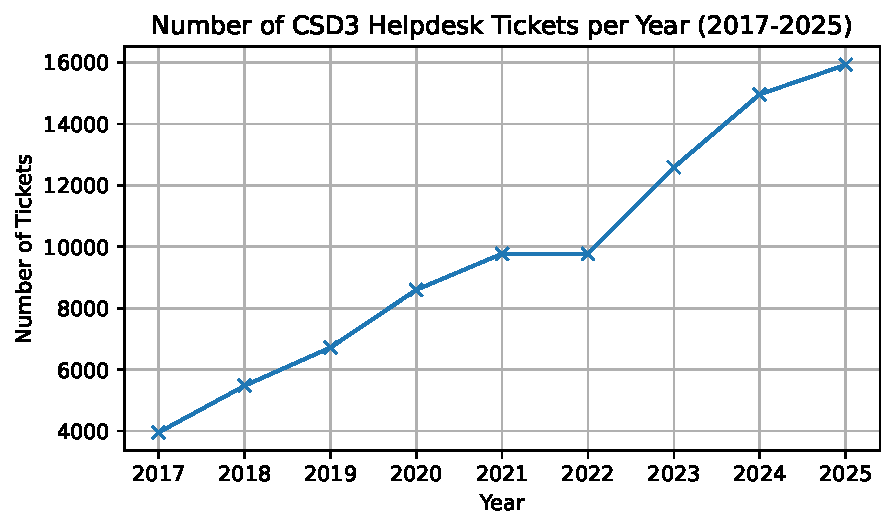
\includegraphics{graphs/ticket_counts.pdf}
    \caption{Annual number of resolved \acs{CSD3} helpdesk tickets from 2017 to 2025. Data sourced from \acs{RCS} support ticket records.}
    \label{fig:ticket-counts}
\end{figure}

Recent work has shown that \ac{RAG} is a promising approach for technical support \ac{QA} because it combines language generation with access to external evidence \citep{AskHPC,lewisRetrievalaugmentedGenerationKnowledgeintensive2020}. However, in heterogeneous support environments, answer quality depends not only on topical relevance, but also on whether the retrieved evidence is authoritative, current, and applicable to the local system state \citep{liYouKnowWhat2024,hwangRetrievalAugmentedGenerationEstimation2025}. In the \ac{CSD3} setting, this matters because local documentation, external package documentation, and historical support tickets play different evidential roles. The central challenge is therefore to retrieve evidence that is not just similar to the query, but suitable for the current \ac{CSD3} context. 

\section{Problem Definition and Scope}
\label{sec:problem}

This dissertation studies evidence-grounded first-response assistance for \ac{CSD3} support queries within a supervised internal workflow. The system is limited to single-hop questions, that is, queries answerable in one retrieval step from text-accessible evidence drawn from local documentation, selected external documentation, and visible ticket content. It does not attempt autonomous resolution and excludes attachment-dependent or multimodal evidence such as screenshots and log files. These boundaries keep the task operationally realistic while allowing later experiments to isolate the effect of heterogeneous-source retrieval and validity-aware reranking. 

\section{Research Questions and Hypotheses}
\label{sec:questions}

To investigate the problems introduced by the heterogeneous evidence base, this project addresses the following research questions (RQ), along with the associated hypotheses (H):

\begin{itemize}
    \item \textbf{RQ1:} \label{rq:1-source} Does combining local \ac{CSD3} documentation with historical support-ticket evidence improve the factual correctness of answers, relative to single-source retrieval?
    \begin{itemize}
        \item \textbf{H1:} Combined retrieval will outperform documentation-only and ticket-only baselines in factual correctness, particularly for case-specific troubleshooting queries for which local documentation and historical resolutions provide complementary evidence.  
    \end{itemize}
    \item \textbf{RQ2:} \label{rq:2-validity} Does validity-aware reranking improve the factual correctness and faithfulness of answers, relative to source-agnostic relevance-based retrieval over the same heterogeneous corpus?
    \begin{itemize}
        \item \textbf{H2:} Validity-aware reranking will outperform source-agnostic retrieval by reducing the selection of outdated, weakly authoritative, or locally inapplicable evidence, with the largest gains on version-sensitive and current-policy queries.
    \end{itemize}
\end{itemize}

A secondary analysis examines whether curated external documentation adds value for software-specific queries beyond the core local evidence base. To answer these questions, this project uses held-out comparisons of source ablations and reranking variants. 

\section{Aim, Objectives, and Success Criteria}
\label{sec:aim}

The principal aim of this project is to design and evaluate an end-to-end \ac{RAG} assistant for use in a supervised \ac{CSD3} support workflow. Within the scope of single-hop, text-accessible user support queries, the project investigates whether combining heterogeneous support evidence with validity-aware retrieval improves the factual correctness and faithfulness of grounded first-response answers. To achieve this aim, the project pursues the following objectives:

\begin{itemize}
    \item \textbf{O1:} To construct a reproducible, queryable support corpus from local \ac{CSD3} documentation, historical support tickets, and selected external documentation, using source-specific preprocessing, chunking, and metadata enrichment. 
    \item \textbf{O2:} To implement an end-to-end \ac{RAG} assistant and baseline retrieval configurations for \ac{CSD3} support queries, capable of producing grounded first-response answers from retrieved evidence. 
    \item \textbf{O3:} To design and integrate a validity-aware retrieval and reranking strategy that uses authority, scope, freshness, version, and status signals to prioritise evidence appropriate to the current \ac{CSD3} environment. 
    \item \textbf{O4:} To develop a benchmark and experimental framework for single-hop \ac{CSD3} support queries, including a fixed development and test split and manually verified benchmark annotations for source requirements and validity sensitivity. 
    \item \textbf{O5:} To evaluate whether heterogeneous-source retrieval and validity-aware reranking improve factual correctness over relevant baselines through controlled ablations, finalist comparisons, manual evaluation, and error analysis. 
\end{itemize}

These objectives are evaluated against three research-facing success criteria. First, the project must provide a convincing held-out answer to whether combining local documentation and historical tickets improves factual correctness over single-source baselines. Second, it must provide a convincing held-out answer to whether validity-aware reranking improves over naive combined retrieval, judged primarily by factual correctness and checked against faithfulness. Third, it must reach a justified conclusion about the role of external documentation for software-specific queries, including whether any benefit is limited or conditional. Supporting implementation, reproducibility, and protocol criteria are operationalised in Chapter~\ref{cha:problem}.

\section{Overview of Evaluation Strategy}
\label{sec:eval_overview}

The evaluation strategy was designed to answer the research questions with minimal selection bias. The benchmark was split into development and held-out test partitions so that generator selection and configuration tuning were separated from final comparison \citep{westphalImprovingModelSelection2019}. The held-out experiments then compare single-source retrieval, naive combined retrieval, validity-aware reranking, and the contribution of external documentation. Factual correctness is the primary metric because the central aim of the project is to improve the correctness of support answers. Faithfulness is used as a guardrail against unsupported generation, while additional retrieval metrics are used diagnostically when comparing retrieval variants. Manual evaluation and error analysis complement automated scoring by identifying user-relevant failure modes and limitations \citep{RAGAS,grittaHumanRankEvalAutomaticEvaluation2024,chenSurfaceMeasuringSelfPreference2025}.

The full experimental protocol is further described in Chapter \ref{cha:methodology}, with results presented in Chapters \ref{cha:results} and \ref{cha:discussion}. 

\section{Report Structure}
\label{sec:structure}

The remainder of this report is structured to move from background and problem definition through to system design, evaluation, results, and conclusions. Chapter~\ref{cha:background} reviews the literature, Chapter~\ref{cha:problem} defines the task, benchmark, and requirements, Chapter~\ref{cha:system-design-implementation} describes the system, Chapter~\ref{cha:methodology} presents the experimental methodology, Chapter~\ref{cha:results} reports the results, Chapter~\ref{cha:discussion} discusses the findings and limitations, and Chapter~\ref{cha:conclusion} concludes. 
\chapter{Background and Related Work}
\label{cha:background}

\section{HPC Support as an Information Retrieval and Question Answering Problem}
\label{sec:support}

\section{Retrieval-Augmented Generation}
\label{sec:rag}

\section{Heterogeneous Support Corpora: Documentation and Tickets}
\label{sec:heterogeneous}

\section{Authority, Freshness, and Validity in Retrieval}
\label{sec:authority-freshness-validity}

\section{Evaluation of RAG Systems}
\label{sec:evaluation}

\section{Failure Modes of Naive Retrieval}
\label{sec:failure-modes}

\section{Gap Analysis and Research Positioning}
\label{sec:gap}
\chapter{Problem Formulation and Requirements}
\label{cha:problem}

\section{Task Definition}
\label{sec:task}

\section{Data Sources and Knowledge Characteristics}
\label{sec:data}

\section{Failure modes of Naive Retrieval}
\label{sec:naive_retrieval_failure}

\section{Functional Requirements}
\label{sec:functional_requirements}

\section{Non-Functional Requirements}
\label{sec:non_functional_requirements}

\section{Ethical, Privacy, and Data-Governance Considerations}
\label{sec:ethical_considerations}
\chapter{System Design and Implementation}
\label{cha:system-design-implementation}

\section{System Overview}
\label{sec:system-overview}

This chapter describes Polaris, a retrieval-augmented assistant designed for supervised \ac{CSD3} support question answering. It implements the design requirements defined in Chapter~\ref{cha:problem} as a modular retrieval-augmented support system. Its architecture separates offline evidence preparation from runtime query handling so that corpus construction, metadata enrichment, retrieval, generation, and auditability can be controlled independently. The system indexes local documentation, external official documentation, and historical support tickets into source distinct stores, with authority and validity metadata used to preserve differences in reliability and operational relevance. This separation is central to Polaris's design, allowing runtime retrieval to combine heterogeneous evidence while still exposing the metadata needed for reviewable support responses. 

\begin{figure}[ht]
    \centering
    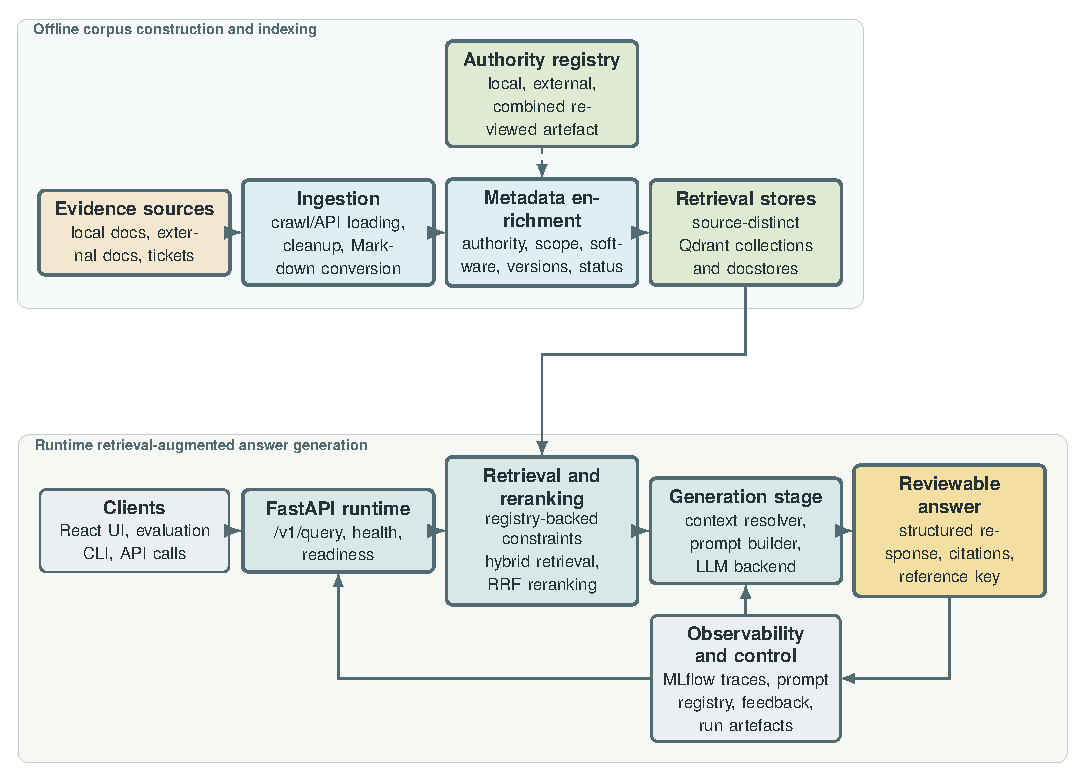
\includegraphics[width=\textwidth]{graphs/polaris_architecture.pdf}
    \caption[High-level architecture of Polaris.]{High-level architecture of Polaris. Offline corpus construction converts local documentation, external official documentation, and resolved support tickets into source-distinct retrieval stores enriched with authority and validity metadata. At runtime, the API coordinates registry-backed query-constraint extraction, multi-collection retrieval, configurable reranking, context resolution, prompt construction, generation, and reviewable evidence-grounded response output.}
    \label{fig:polaris-architecture}
\end{figure}

Figure~\ref{fig:polaris-architecture} separates Polaris into offline corpus construction and runtime answer generation. Offline construction ingests the evidence sources, converts them into a consistent representation, enriches them with metadata, and indexes them into source-distinct Qdrant collections and document stores \citep{CollectionsQdrant}. At runtime, the FastAPI service coordinates registry-backed query interpretation, multi-collection retrieval, reranking, context resolution, prompt construction, LLM generation, and response packing. The observability layer records traces, prompt versions, feedback, and run artefacts, supporting reproducibility and making system behaviour auditable during evaluation and debugging. 

\begin{figure}[ht]
    \centering
    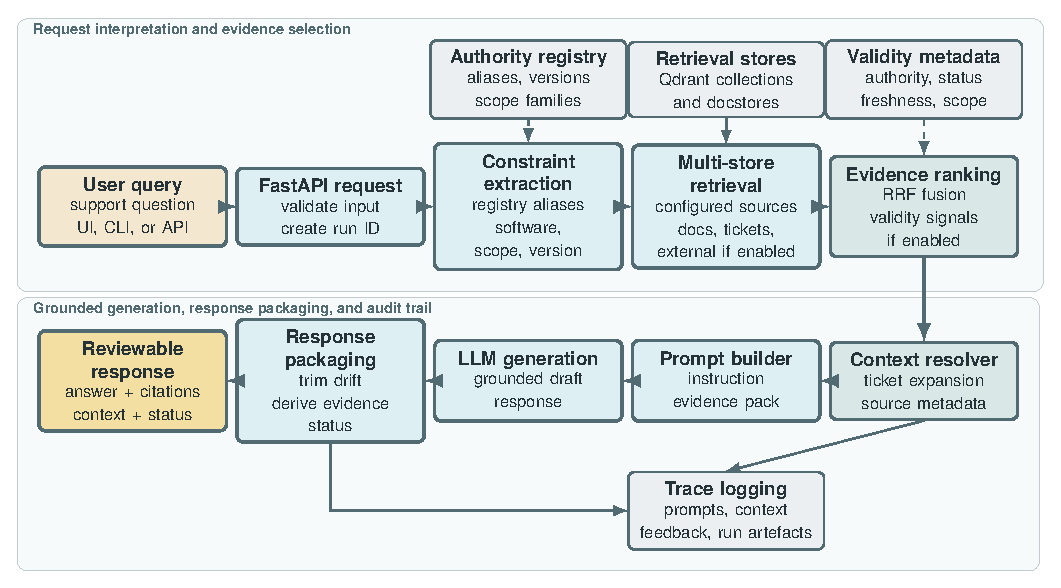
\includegraphics[width=\textwidth]{graphs/polaris_query_flow.pdf}
    \caption[Runtime query flow in Polaris.]{Runtime query flow in Polaris. A user query is validated by the API, converted into registry-backed retrieval constraints, matched against configured source-distinct stores, fused and reranked, resolved into final evidence contexts, passed to the generation prompt, and repackaged with output cleanup, evidence status, and trace outputs before a reviewable response is returned.}
    \label{fig:polaris-query-flow}
\end{figure}

Figure~\ref{fig:polaris-query-flow} illustrates how an individual user query moves through the system. A query is first validated by the API and associated with runtime tracing information. The system then extracts registry-backed constraints, such as software, version, scope, and intent signals, before retrieving evidence from the configured source-distinct stores. Retrieved candidates are then fused and ranked using \ac{RRF}, with validity signals available where enabled. The selected evidence is resolved into final contexts, rendered into the generation prompt, and passed to the LLM. The generated answer is then packaged by trimming output drift, deriving an evidence status from the retrieved context count, and logging the relevant outputs for auditability.  

The remainder of this chapter decomposes this overview into the main implementation decisions and design trade-offs made during Polaris's development. 

\section{Baseline Systems}
\label{sec:baseline-systems}

This project implements a series of baseline systems to evaluate the impact of specific design choices in Polaris. Each baseline system is a controlled comparison version of the main Polaris system, with specific design choices removed to isolate their effects. The generator, API pipeline, prompt format, and evaluation protocol are held constant across all systems to ensure that any observed differences in performance can be attributed to the design choices being evaluated.

Two baseline systems are implemented with respect to \hyperref[rq:1-source]{Research Question 1}. The first, \texttt{docs\_only}, is a documentation-only system that retrieves from the local \ac{CSD3} documentation collection. It measures how far local documentation alone can support user queries. The second, \texttt{tickets\_only}, is a ticket-only system that retrieves from the historical support ticket collection. It measures how far historical resolutions alone can support user queries. Comparing these baselines to the full Polaris system, which retrieves from both sources, allows us to evaluate whether combining heterogeneous evidence improves answer quality.

A single baseline system is implemented with respect to \hyperref[rq:2-validity]{Research Question 2}. This baseline, \texttt{naive\_combined}, uses both local documentation and historical tickets with standard \ac{RRF} retrieval, but without validity-aware reranking. This allows us to evaluate whether the validity-aware reranking design in Polaris improves answer quality. Further retrieval variants are also implemented as part of an ablation study, however these are not treated as formal baselines. 

\section{Corpus Ingestion and Representation}
\label{sec:corpus-ingestion-representation}

This section describes how the raw evidence sources are ingested into retrieval-ready evidence units. In this project, local \ac{CSD3} documentation, external documentation, and resolved support tickets are ingested through separate pipelines, but preserved source boundaries so that later source-aware retrieval and reranking remains explicit. 

In this dissertation, chunking refers to splitting a longer source document into smaller bounded text units that can be independently embedded, indexed, and retrieved. This choice matters because whole-document retrieval is too coarse, while overly small chunks may lose important context \citep{wangDocumentSegmentationMatters2025}. 

For the documentation sources, the ingestion pipeline first preprocesses the HTML pages, then converts them into a markdown-normalised representation before token-based chunking. Markdown conversion is used because the source material originates from heterogeneous HTML structures, whereas markdown preserves useful structure such as headings, lists, code blocks, and links in a consistent text format while removing much of the presentation-specific noise of raw HTML. A token-based chunking strategy is then applied because documentation pages are primarily informational rather than conversational. As a result, a fixed token budget provides stable retrieval units while retaining enough local context for procedural and configuration-oriented queries. 

For historical support tickets, the ingestion pipeline first queries the Atlassian Jira API for resolved tickets, converts the JSON content into a structured transcript format, and then applies a dialogue-based chunking strategy. Each ticket is represented using its key, summary, status, available timestamps, initial description, and subsequent conversational exchange. Speaker roles are derived from Jira user fields and preserved at the message level. Furthermore, ticket-level status and timing information are retained as metadata rather than embedded directly into every chunk. A dialogue-based chunking strategy is used because important support evidence often spans a short sequence of messages rather than a single isolated passage. In the final system, chunks are bounded by a fixed token budget and a maximum turn count [OVERLAP???]. Retrieved ticket chunks are then used to identify relevant tickets, after which the corresponding full ticket transcript is resolved for generation so that retrieval remained fine-grained while answer generation included the broader problem-resolution context.  

The final chunking settings, including both chunk size and overlap, are selected empirically. These results are discussed further in Section~\ref{sec:chunking-tuning}.

TODO: add final settings here.

\section{Authority Registry and Metadata Extraction}
\label{sec:authority-registry-metadata-extraction}

Once the source documents have been converted into retrieval-ready representations, the system requires a structured authority layer to identify the technical entities they mention and to attach the metadata needed for later retrieval decisions. This is implemented as an offline authority registry that normalises systems, partitions, services, software packages, modules, and toolchains together with their associated scope, version, and lifecycle information. During ingestion, this registry is used to enrich source records before their metadata is propagated to the retrieval chunks. 

To ensure deterministic and auditable metadata enrichment, the authority registry is built offline, prior to runtime query handling. Local \ac{CSD3} documentation, and where configured, registered external documentation sources are first converted into separate markdown-normalised corpora. These corpora are scanned for candidate entities, which are then merged into normalised registry entries so that repeated mentions across pages map to a single stable definition. Ambiguous aliases or conflicting lifecycle statuses are not resolved silently. Instead, they are added to a review queue for manual inspection. The resulting artefacts are persisted as stable JSON along with build metadata such as source scope and extraction version, supporting traceability and reproducibility. Table~\ref{tab:authority-registry-summary} summarises the entity categories captured by the registry and the main classes of information stored for each entry. 

\begin{longtable}{@{}p{0.20\textwidth} p{0.28\textwidth} p{0.44\textwidth}@{}}
\caption[Summary of the authority registry.]{Summary of the entity categories and metadata stored in the Polaris authority registry.}
\label{tab:authority-registry-summary} \\
\toprule
Registry aspect & Contents & Why it is stored \\
\midrule
\endfirsthead

\toprule
Registry aspect & Contents & Why it is stored \\
\midrule
\endhead

\bottomrule
\endfoot

Entity categories & systems, partitions, services, software, modules, toolchains & Normalises the main technical entity types that Polaris must reason about across documentation and tickets. \\

Identity fields & canonical name, aliases & Links different surface forms to the same underlying entity during matching and query interpretation. \\

Scope, lifecycle, and version fields & source scope, lifecycle status, known versions & Supports source-aware retrieval and version-sensitive reasoning. \\

Provenance fields & source document, heading path, evidence span & Makes extracted metadata traceable to the originating source and section. \\

Audit fields & extraction method, review state & Supports reproducibility and manual review of ambiguous or conflicting cases. \\

\end{longtable}

For the documentation sources, metadata extraction is mainly done by matching the document's source identity against registry entries so that each chunk inherits the entity information associated with its originating document. On the other hand, for the ticket sources, metadata extraction is text-driven: ticket content is scanned using alias matching, \texttt{module load} parsing, and version mention extraction. The resulting matches are then resolved against the same authority registry. This process attaches authority, entity, scope, validity, freshness, provenance, and governance signals to each retrieval unit, with the complete field-level schema summarised in Appendix~\ref{app:authority-metadata-fields}. Using the same registry for both documentation and ticket metadata extraction ensures that they are both interpreted through one consistent set of entity definitions, rather than source-specific rules. 

This metadata is not stored solely for description, but also to support later runtime decisions. Since each retrieval unit carries explicit authority, scope, version, validity, and provenance signals, the same registry-backed representation can be used for query constraint parsing, source-aware retrieval, and validity-aware reranking. The authority layer therefore acts as a bridge between offline corpus preparation and online answer generation. Furthermore, the authority layer also improves auditability, since retrieved evidence can be traced back to its original source, matched entities, and extraction context, making errors easier to inspect during evaluation and debugging. 

\section{Validity-Aware Reranking Design}
\label{sec:validity-aware-reranking-design}

As discussed in Chapter~\ref{cha:background}, semantically relevant evidence may still be unsuitable if it is less authoritative, outdated, or locally inapplicable \citep{liYouKnowWhat2024,hwangRetrievalAugmentedGenerationEstimation2025}. To address this, this project does not treat retrieval as a purely relevance-based problem over a flattened homogeneous corpus. Instead, initial relevance-based semantic retrieval is followed by a validity-aware reranking stage that uses the attached authority and validity metadata to promote more suitable evidence. This design allows the system to still leverage relevance signals while also accounting for the heterogeneous nature of the evidence base.

After query constraints have been derived, the system retrieves an initial set of candidates from source-distinct retrievers, and merges them within a multi-collection retrieval stage. The initial merged ordering is formed using \ac{RRF}, which provides a stable rank-based fusion mechanism across the heterogeneous sources \citep{cormackReciprocalRankFusion2009}. Validity-aware reranking is applied on top of the initial semantic ordering, rather than replacing semantic retrieval altogether. The semantic relevance-only fused ranking corresponds to the \texttt{naive\_combined} baseline introduced in Section~\ref{sec:baseline-systems}, and serves as the direct implementation comparator for the proposed reranking design. 

As illustrated in Figure~\ref{fig:polaris-reranking}, the validity-aware reranker begins with the normalised semantic base score derived from the \ac{RRF} ordering. The final reranking score is formed by taking this normalised semantic base and adding weighted contributions from the structured metadata attached during ingestion. These contributions reflect source authority, exact scope match, software match, scope-family match, version match, lifecycle status, and relative freshness. This allows the reranking stage to prefer evidence that is not only topically relevant, but also more authoritative, current, and locally applicable to the active support query. The exact weights and value mappings are configuration-driven rather than hard-coded, so that the scoring policy remains explicit, tunable, and reproducible. The exact weights used by the system were tuned empirically, with the final tuned configuration described further in Section~\ref{sec:validity-reranker-tuning}.

\begin{figure}[ht]
    \centering
    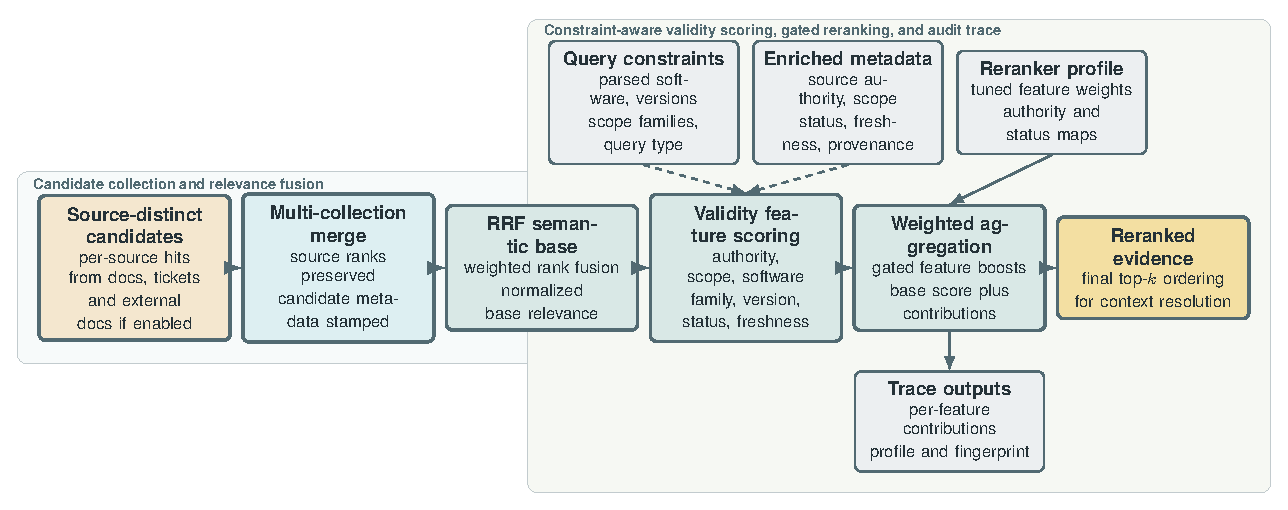
\includegraphics[width=\textwidth]{graphs/polaris_reranking.pdf}
    \caption[Validity-aware reranking in Polaris.]{Validity-aware reranking in Polaris. Source-distinct candidates are merged and fused into an RRF semantic base, then adjusted using query-aware validity features derived from registry-backed constraints, enriched metadata, and the configured reranker profile before final evidence selection.}
    \label{fig:polaris-reranking}
\end{figure}

These validity signals are not applied blindly to every query. Instead, the reranker uses the derived query constraints to control how individual metadata features should behave. This is particularly important for software-constrained queries, where a broad scope-family match could otherwise promote evidence that refers to the correct platform family but not the relevant software package. In such cases, the scope-family boosts are gated unless the candidate also satisfies the required software match, and specialised family variants are prevented from receiving an inappropriate generic boost when the exact variant is not actually requested. On the other hand, for non-software operational queries scope-family similarity can provide a useful positive signal. These safeguards are intended to reduce false promotion of evidence that is broadly related but operationally inappropriate for the active query. 

The reranking design was also implemented to support controlled evaluation. The active reranker configuration is therefore persisted as a structured profile and fingerprint, and these are logged alongside retrieval traces and final outputs so that ranking behaviour can be reconstructed across runs. This makes it possible to compare reranker variants under a controlled evaluation protocol. The tuning procedure is described in Section~\ref{sec:validity-reranker-tuning}, and the contribution of individual validity signals is evaluated in Section~\ref{sec:validity-signal-ablation}.

\section{Prompt and Generation Design}
\label{sec:prompt-generation-design}

In this project, the generation stage is designed around producing grounded, operationally useful, and reviewable support responses. A fixed prompt template is used across all system variants, allowing the impact of retrieval and reranking design choices to be evaluated without the confounding effects of prompt changes. The prompt is designed to match the gold standard ticket format in the evaluation dataset to improve comparability with the reference answers and allow for easier manual inspection. The prompt also includes few-shot examples detailing both a normal example, and an example containing insufficient evidence. This teaches the target response structure and citation style, while also providing a reference for how to handle uncertain questions and ask for follow-up questions when evidence is weak \citep{brownLanguageModelsAre2020}.

The prompt used contains a system instruction defining the model as a \ac{CSD3} support analyst and explicitly prohibiting the generation of unsupported facts, paths, policies, or actions. It also includes a user section, which renders the query along with numbered retrieved evidence contexts and stable document IDs. The expected output format is then defined, listing mandatory section headers. The use of fixed sections allows for outputs that are easier to review, compare, and reuse in a supervised support workflow. The user section also enforces numeric citation on factual paragraphs and non-trivial actions. This improves traceability from claims back to the retrieved evidence and reduces unsupported generation \citep{gaoEnablingLargeLanguage2023}. Furthermore, the prompt ends with a mandatory \texttt{REFERENCE KEY} mapping the used citation numbers to the stable document IDs. This further improves the traceability of generated answers, allowing reviewers to easily inspect the cited evidence and compare it against the generated claims. 

In the context of \ac{HPC} support, a plausible but operationally incorrect answer is worse than no answer at all. As a result, when retrieved context is missing or conflicting, the prompt requires the  model to state uncertainty, choose the safest next step, and ask for concise follow-up questions rather than guessing. Furthermore, a post-processing step is applied to the generated output to trim any output drift and rebuild the \texttt{REFERENCE KEY} from the citations actually used in the final answer. This prevents any uncited or hallucinated reference mappings from being included in the final output. 

The final generator configuration used \texttt{meta-llama/Llama-3.3-70B-Instruct} with a $2048$-token output limit, temperature $0.8$, and top-p $0.9$. These settings provided a practical balance between bounded, reviewable responses, and enough linguistic flexibility to produce natural support-style text. 

\section{API, Tooling, and Observability}
\label{sec:api-tooling-observability}

\section{User Interface and Interaction Design}
\label{sec:user-interface-interaction-design}

\section{Verification and Software Testing}
\label{sec:verification-testing}

\section{Design Trade-offs}

%TODO - add a UI subsection
%TODO - make sure to define all systems

\chapter{Experimental Methodology}
\label{cha:methodology}

\section{Evaluation Goals}
\label{sec:evaluation-goals}

\section{Development and Test Split Discipline}
\label{sec:dev-test-split}

\section{Benchmark Construction and Characterisation}
\label{sec:benchmark-construction-characterisation}

\section{Frozen Backbone Decisions}
\label{sec:frozen-backbone-decisions}

\section{Metric Hierarchy and Decision Rules}
\label{sec:metric-hierarchy-decision-rules}

\section{Development-Phase Tuning Protocol}
\label{sec:dev-phase-tuning-protocol}

\subsection{Generator Selection}
\label{sec:generator-selection}

\subsection{Chunking Tuning}
\label{sec:chunking-tuning}

\subsection{Retrieval-Mode Pilot}
\label{sec:retrieval-mode-pilot}

\subsection{Shared Retrieval Budget Tuning}
\label{sec:shared-retrieval-budget-tuning}

\subsection{Validity-Reranker Tuning}
\label{sec:validity-reranker-tuning}

\section{Final Test-Set Experiments}
\label{sec:final-test-set-experiments}

\subsection{Source Ablation}
\label{sec:source-ablation}

\subsection{Validity-Signal Ablation}
\label{sec:validity-signal-ablation}

\subsection{External-Document Scope Ablation}
\label{sec:external-document-scope-ablation}

\subsection{Tuned-Finalist Comparison}
\label{sec:tuned-finalist-comparison}

\section{Manual Evaluation Protocol}
\label{sec:manual-evaluation-protocol}

\section{Error Analysis Protocol}
\label{sec:error-analysis-protocol}

\section{Reproducibility and Stability Controls}
\label{sec:reproducibility-stability-controls}
\chapter{Results}
\label{cha:results}

\section{Development-Phase Selection Results}
\label{dev-results}

\section{Overview of Main Test-Set Results}
\label{sec:overview-main-test-set-results}

\section{Controlled Ablation Results}
\label{sec:controlled-ablation-results}

\subsection{Source Ablation}
\label{sec:source-ablation}

\subsection{Validity-Signal Ablation}
\label{sec:validity-signal-ablation}

\subsection{External-Document Scope Ablation}
\label{sec:external-document-scope-ablation}

\section{Practical Comparison Results}
\label{sec:practical-comparison-results}

\subsection{Tuned-Finalist Comparison}
\label{sec:tuned-finalist-comparison}

\section{Manual Evaluation Results}
\label{sec:manual-evaluation-results}

\section{Error Analysis Results}
\label{sec:error-analysis-results}

\section{Stability and Robustness Results}
\label{sec:stability-robustness-results}

\chapter{Discussion and Critical Appraisal}
\label{cha:discussion}

\section{Answers to the Research Questions}
\label{sec:answer-research-questions}

\section{What Improved and Why}
\label{sec:what-improved-why}

\section{Comparison with Prior Work}
\label{sec:comparison-prior-work}

\section{Where the System Still Fails}
\label{sec:where-system-still-fails}

\section{Threats to Validity}
\label{sec:threats-to-validity}

\section{Review of the Project Plan}
\label{sec:review-project-plan}
\chapter{Conclusion and Future Work}
\label{cha:conclusion}

\section{Summary of Contributions}
\label{sec:summary-contributions}

\section{Main Findings}
\label{sec:main-findings}

\section{Limitations}
\label{sec:limitations}

\section{Future Work}
\label{sec:future-work}

  \bibliography{refs}    % this causes the references to be listed

\bibliographystyle{IEEEtranN}
%% the bibliography style determines the format  in which both citations and references are printed,
%% other possible values are plain and abbrv
%%
%% If you want more control of the format of your citations you might want to take a look at
%% natbib.sty, which should be part of any standard LaTeX installation
%%
%% University regulations simply require that your citation style be consistent, so see what style
%% your supervisor recommends.

% Appendices start here

\appendix
\chapter{Approved External Documentation Sources}
\label{app:external-sources}

This appendix lists the approved external documentation source families included in the frozen external documentation snapshot used for parameter tuning and final evaluation. These sources were selected as stable, official documentation sources relevant to the \ac{CSD3} support domain. The list documents the approved source boundaries used for corpus construction. 

\begingroup
\footnotesize
\setlength{\tabcolsep}{4pt}
\renewcommand{\arraystretch}{1.1}

\begin{longtable}{p{2.5cm} p{4.4cm} p{6.1cm}}
\caption{Approved external documentation source families included in the frozen external documentation snapshot used for parameter tuning and final evaluation.}
\label{tab:approved-external-sources} \\

\hline
Source & Approved scope & Support relevance \\
\hline
\endfirsthead

\multicolumn{3}{l}{\textit{Table \thetable{} continued from previous page}} \\
\hline
Source & Approved scope & Support relevance \\
\hline
\endhead

\hline
\multicolumn{3}{r}{\textit{Continued on next page}} \\
\endfoot

\hline
\endlastfoot

Slurm (software) &
\url{https://slurm.schedmd.com/} &
Scheduler usage, job submission, resource requests, and runtime behaviour. \\

CUDA (toolchain) &
\url{https://docs.nvidia.com/cuda/} &
GPU programming, CUDA runtime, and accelerator-specific software issues. \\

Intel oneAPI (toolchain) &
\url{https://www.intel.com/content/www/us/en/docs/oneapi/} &
Intel compilers, build configuration, optimisation, and environment setup. \\

Open MPI (toolchain) &
\url{https://docs.open-mpi.org/en/main/}; \url{https://docs.open-mpi.org/en/v5.0.x/} &
MPI execution, communication behaviour, and version-sensitive runtime detail. \\

PyTorch (software) &
\url{https://docs.pytorch.org/docs/stable/} &
Distributed training, GPU use, Python environments, and framework-specific queries. \\

TensorFlow (software) &
\url{https://www.tensorflow.org/api_docs}; \url{https://www.tensorflow.org/guide} &
Framework APIs, environment setup, and model-execution issues. \\

GROMACS (software) &
\url{https://manual.gromacs.org/documentation/current/} &
Molecular simulation usage, command syntax, and software-specific troubleshooting. \\

LAMMPS (software) &
\url{https://docs.lammps.org/stable/} &
Input syntax, package behaviour, and software-specific execution detail. \\

OpenFOAM (software) &
\url{https://doc.cfd.direct/openfoam/user-guide-v13/} &
Solver usage, case setup, and computational fluid dynamics support issues. \\

OpenMM (software) &
\url{https://docs.openmm.org/latest/userguide/} &
GPU-accelerated molecular simulation, software usage, and configuration questions. \\

Intel MPI (toolchain) &
\url{https://www.intel.com/content/www/us/en/docs/mpi-library/developer-guide-linux/2021-16/} &
MPI runtime behaviour, communication libraries, and parallel-execution troubleshooting. \\

SingularityCE (software) &
\url{https://docs.sylabs.io/guides/latest/user-guide/} &
Container execution, bind mounts, and software-environment portability on HPC systems. \\

Spack (software) &
\url{https://spack.readthedocs.io/en/latest/} &
Package installation, environment composition, and reproducible build workflows. \\

\end{longtable}
\endgroup

The approved scope for each source was controlled through the external source registry by restricting crawls to specified domains and included URL prefixes, while excluding archive, release-note, API, PDF, or otherwise misaligned subtrees where appropriate. This ensures that the external corpus remained focused on stable, official, and support-relevant documentation rather than becoming an unrestricted crawl of general web content. 
\chapter{Benchmark Taxonomy Label Definitions}
\label{app:benchmark-taxonomy-labels}

This appendix defines the multi-label taxonomy used to annotate benchmark queries for later subgroup analysis. Each field captures a distinct property of the query or of the minimum evidence conditions required for a correct answer. 

\newcommand{\topcode}[1]{\parbox[t]{\linewidth}{\raggedright\ttfamily #1}}
\newcommand{\toptext}[1]{\parbox[t]{\linewidth}{\raggedright #1}}

\begingroup
\footnotesize
\setlength{\tabcolsep}{4pt}
\renewcommand{\arraystretch}{1.15}

\begin{longtable}{>{\raggedright\arraybackslash}p{2.6cm}
                  >{\raggedright\arraybackslash}p{3.3cm}
                  >{\raggedright\arraybackslash}p{3.6cm}
                  >{\raggedright\arraybackslash}p{4.8cm}}
\caption{Benchmark taxonomy label definitions and allowed values.}
\label{tab:benchmark-taxonomy-labels} \\

\hline
Field & What it captures & Allowed values & Annotation rule \\
\hline
\endfirsthead

\multicolumn{4}{l}{\textit{Table \thetable{} continued from previous page}} \\
\hline
Field & What it captures & Allowed values & Annotation rule \\
\hline
\endhead

\hline
\multicolumn{4}{r}{\textit{Continued on next page}} \\
\endfoot

\hline
\endlastfoot

\topcode{source\_\newline needed} &
\toptext{The minimum evidence class needed for a correct answer} &
\topcode{docs\newline tickets\newline both} &
\toptext{Labels describe the task, not the current retrieval result or the current vector-store contents. Assign the minimum evidence class required for a correct answer.} \\

\topcode{docs\_scope\_\newline needed} &
\toptext{Which class of official documentation is authoritative when documentary evidence is needed} &
\topcode{local\_official\newline external\_official\newline local\_and\_external\newline none} &
\toptext{Use \texttt{none} only when \texttt{source\_needed=tickets}. Queries with \texttt{source\_needed=docs} or \texttt{both} must not use \texttt{none}.} \\

\topcode{validity\_\newline sensitive} &
\toptext{Whether correctness depends on current system, partition, service, workflow, or compatibility truth} &
\topcode{yes\newline no} &
\toptext{Mark \texttt{yes} when current local operational truth is central to correctness; mark \texttt{no} when the answer is sufficiently stable.} \\

\topcode{attachment\_\newline dependent} &
\toptext{Whether visible text alone is sufficient, or whether unseen attachments materially determine correct handling} &
\topcode{yes\newline no} &
\toptext{Mark \texttt{yes} when screenshots, logs, uploaded documents, or other unseen attachments materially affect the correct first response.} \\

\topcode{query\_type} &
\toptext{The broad problem family represented by the query} &
\topcode{local\_operational\newline software\_version\newline general\_how\_to} &
\toptext{Assign the dominant problem family: local service truth, version-sensitive software or toolchain issues, or stable procedural guidance.} \\

\topcode{version\_\newline sensitive} &
\toptext{Whether correctness depends materially on a software or toolchain version} &
\topcode{yes\newline no} &
\toptext{Mark \texttt{yes} when version differences could change the correct guidance or resolution.} \\

\topcode{system\_scope\_\newline required} &
\toptext{Whether correctness depends on a particular system, service, partition, or platform} &
\topcode{yes\newline no} &
\toptext{Mark \texttt{yes} when the answer would differ materially across systems or execution environments.} \\

\end{longtable}
\endgroup

Where multiple interpretations were possible, labels were assigned according to the minimum evidence needed for a correct and locally applicable first-response answer. 
\chapter{Authority Metadata Fields}
\label{app:authority-metadata-fields}

Table~\ref{tab:authority-metadata-fields} summarises the main metadata fields attached during ingestion. These fields are derived from the authority registry and associated preprocessing steps, and are later used to support retrieval, reranking, provenance tracking, and reviewability.

\begin{longtable}{@{}p{0.24\textwidth} p{0.30\textwidth} p{0.38\textwidth}@{}}
\caption[Authority metadata fields attached during ingestion.]{Authority metadata fields attached during ingestion in Polaris.}
\label{tab:authority-metadata-fields} \\
\toprule
Field & Description & Role in the system \\
\midrule
\endfirsthead

\toprule
Field & Description & Role in the system \\
\midrule
\endhead

\bottomrule
\endfoot

\texttt{source\_authority} & Encodes the authority class of the source, such as local official documentation, external official documentation, or ticket memory. & Supports source-aware retrieval and allows later stages to distinguish evidence by reliability class. \\

\texttt{authority\_tier} & Numeric authority level derived from the source authority class. & Provides a compact ranking signal for reranking and diagnostic analysis. \\

\texttt{system\_names} & Normalised system entities matched to the record. & Identifies which cluster or platform the evidence refers to. \\

\texttt{partition\_names} & Normalised partition entities matched to the record. & Supports queries involving scheduler partitions or node classes. \\

\texttt{service\_names} & Normalised service entities matched to the record. & Helps capture operational services such as portals or interfaces. \\

\texttt{scope\_family\_names} & Higher-level scope groupings inferred from matched entities or text patterns. & Allows broader retrieval and reranking decisions beyond exact entity matches. \\

\texttt{software\_names} & Normalised software entities matched to the record. & Identifies the main software packages discussed in the evidence. \\

\texttt{software\_versions} & Version mentions associated with matched software entities. & Supports version-sensitive retrieval and reranking. \\

\texttt{module\_names} & Matched module identifiers extracted from the content. & Helps interpret module-based software references in tickets and documentation. \\

\texttt{toolchain\_names} & Normalised toolchain entities matched to the record. & Distinguishes compiler or build-stack context where relevant. \\

\texttt{toolchain\_versions} & Version mentions associated with matched toolchain entities. & Supports toolchain-specific matching and version alignment. \\

\texttt{official\_doc\_matches} & Structured record of registry entity matches back to official documentation. & Preserves documentary support for matched entities and enables later auditability. \\

\texttt{validity\_status} & Aggregated lifecycle status inferred from matched registry entities, such as current, maintenance, legacy, or end-of-life. & Supplies a direct validity signal for reranking and review. \\

\texttt{validity\_hint} & Structured diagnostic summary of matched status evidence. & Preserves a richer explanation of validity beyond a single label. \\

\texttt{freshness\_hint} & Timestamp-like recency cue derived from available metadata fields. & Supports recency-sensitive ranking and later analysis of stale evidence. \\

\texttt{privacy\_flags} & Flags indicating the presence of potentially sensitive patterns such as email addresses, IP addresses, or filesystem paths. & Supports governance and safer handling of retrieved ticket evidence. \\

\texttt{provenance} & Structured provenance record including enrichment version, registry artifact path, extraction version, and matched entity identifiers. & Makes enrichment outputs reproducible, traceable, and reviewable. \\

\end{longtable}


\end{document}
